%%%%%%%%%%%%%%%%%%%% book.tex %%%%%%%%%%%%%%%%%%%%%%%%%%%%%
%
% sample root file for the chapters of your "monograph"
%
% Use this file as a template for your own input.
%
%%%%%%%%%%%%%%%% Springer-Verlag %%%%%%%%%%%%%%%%%%%%%%%%%%


% RECOMMENDED %%%%%%%%%%%%%%%%%%%%%%%%%%%%%%%%%%%%%%%%%%%%%%%%%%%
\documentclass[graybox,envcountchap,sectrefs]{svmono}

% choose options for [] as required from the list
% in the Reference Guide

%\usepackage{mathptmx}
%\usepackage{helvet}
%\usepackage{courier}
%
\usepackage{type1cm}         

\usepackage{makeidx}         % allows index generation
\usepackage{graphicx}        % standard LaTeX graphics tool
                             % when including figure files
\usepackage{multicol}        % used for the two-column index
\usepackage[bottom]{footmisc}% places footnotes at page bottom

\usepackage{newtxtext}       % 
\usepackage{newtxmath}       % selects Times Roman as basic font

% see the list of further useful packages
% in the Reference Guide

\makeindex             % used for the subject index
                       % please use the style svind.ist with
                       % your makeindex program

%%%%%%%%%%%%%%%%%%%%%%%%%%%%%%%%%%%%%%%%%%%%%%%%%%%%%%%%%%%%%%%%%%%%%

\graphicspath{{./}{images/}}

\begin{document}

\author{Author name(s)}
\title{Book title}
\subtitle{-- Monograph --}
\maketitle

\frontmatter%%%%%%%%%%%%%%%%%%%%%%%%%%%%%%%%%%%%%%%%%%%%%%%%%%%%%%


%%%%%%%%%%%%%%%%%%%%%%% dedic.tex %%%%%%%%%%%%%%%%%%%%%%%%%%%%%%%%%
%
% sample dedication
%
% Use this file as a template for your own input.
%
%%%%%%%%%%%%%%%%%%%%%%%% Springer %%%%%%%%%%%%%%%%%%%%%%%%%%


\chapter*{Dedication}
\textit{To my first-born daughter, Alyssa Marie - You are the moment everything changed. The day you were born and I first held you in my arms was the day I learned the true meaning of unconditional love. You made me a mother and becoming your mother gave me a purpose that I desperately craved in my life. You have taught me grace through challenge, joy in the smallest moments, and pride beyond measure. You inspire me to believe in myself and to be the best version of myself. Through you, I live vicariously. You are my guide light, my motivation and the reason why I dream bigger. You are my calm, my courage, and my constant reminder of the love that never ends. I see the best of me in you and everything I strive to become.
}


\textit{To my son, Jayden Christopher, you are my rainbow that came after the storm, the light that followed my darkest days. After an unimaginable loss, you arrived and brought healing that I did not know was possible. Your existence is a promise fulfilled, a prayer answered, and a symbol of hope that love always finds its way back. You are my calm, my rock, and my quiet strength. Always looking out for me, always reminding me to keep going, whether it is nudging me to get up for work or simply standing beside me with that knowing heart of yours. You are my safe place, my gentle guide, and the reminder that from pain comes beauty and from heartbreak comes joy. I thank the universe every day for you. You didn't just fill a void - you built something whole and unshakable in its place.
}


\textit{To my baby, Damien Robert - my fierce little heart. You completed our family with your fire, charm, and your endless hugs. You are my firecracker, my light, my "spelling turtle," and my laughter. From the moment you entered my life, you have filled it with boundless energy, affection, and joy. Your imagination is wild and beautiful, your hugs are healing, and your love is pure magic for my soul. You remind me every day to live in moment, to laugh loudly, and to love without limits. You complete our family in ways only you could, and I am endlessly grateful for the spark you bring into my world. You are my sunshine, my strength, and my sweetest adventure. Watching you grow is one of my life's greatest joys.
}

\textit{To my Mother, my Father, and my brother - your love is the foundation of everything I am. You have lifted me through my lowest moments and cheered me on through every victory and were there in my corner for every loss. Mom, your warmth and compassion live in the everything I do. Dad, your strength and steady presence give me courage to chase dreams bigger than myself. And to my brother - your loyalty, humor, and unspoken understanding have kept me grounded when life felt too heavy. Thank you for standing by me, for believing in me, and for loving me unconditionally even when I didn't have the words to ask for it. This journey is ours - always.
}
\textit{And finally, to You, Dear Reader - Thank you for stepping into my world - where curiosity meets code, where defense is an art, and where knowledge becomes your greatest weapon. To all the new and upcoming, aspiring ethical hackers, to all the seasoned defenders, and to everyone else in between - if you're someone drawn to the power of mystery, the pursuit of knowledge, and a thirst to question everything, this book was written with you in mind. May these pages challenge you, sharpen your skills, and ignite the fire to keep pushing yourself to learn. May you find not just techniques, but purpose - not just exploits, but ethics and guidance. You are the reason this journey matters. Thank you for taking a chance on this book. Now go - learn boldly, defend fiercely, and hack with purpose and honor.
}
Stay safe out there.
All my best.
Stay Safe • Stay Vigilant • Stay Informed
\include{author/foreword}
%%%%%%%%%%%%%%%%%%%%%%preface.tex%%%%%%%%%%%%%%%%%%%%%%%%%%%%%%%%%%%%%%%%%
% sample preface
%
% Use this file as a template for your own input.
%
%%%%%%%%%%%%%%%%%%%%%%%% Springer %%%%%%%%%%%%%%%%%%%%%%%%%%

\preface

%% Please write your preface here
\emph{Master of Your Domain: Hacking and Defending Active Directory (AD) for Ethical Hackers.tex} is a practical exploration of how today's modern Active Directory (AD) environments are breached, abused, and defended in the real-world. This book was written for aspiring and seasoned ethical hackers, red and blue teamers, penetration testers, defenders, and anyone who wants to understand the true dynamics of modern Windows network compromise - beyond theory, beyond checklists.
Active Directory remains one of the most targeted and misunderstood components in enterprise cyber security. It's vast, complex, and oftentimes misconfigured. For attackers, it's a playground - a goldmine. For defenders, it's a battlefield in the truest sense. This book aims to arm you with both perspectives of both offensive and defensive cyber security. You'll find detailed coverage of post-exploitation tactics, including certificate abuse (e.g., Golden Tickets), persistence techniques, lateral movement, privilege escalation, and the tools used and methods in which to attack and defend the Kerberos authentication protocol. But more than just technical content, this book emphasizes mindset: how an attacker thinks when they're inside, undetected, and methodically deciding their next move. Understanding that psychology is just as critical as knowing the tools.
Each chapter is based on real-world engagements and lessons learned the hard way. No two networks are the same - but patterns emerge, and opportunities repeat themselves. The goal of this book is to help you recognize those opportunities. Whether you are breaking in, or locking things down.
To those who supported the long hours, reviewed the raw material, and challenged my thinking - thank you. This book wouldn't exist without your input, insight, and encouragement.


A preface\index{preface} is a book's preliminary statement, usually written by the \textit{author or editor} of a work, which states its origin, scope, purpose, plan, and intended audience, and which sometimes includes afterthoughts and acknowledgments of assistance. 

When written by a person other than the author, it is called a foreword. The preface or foreword is distinct from the introduction, which deals with the subject of the work.

Customarily \textit{acknowledgments} are included as last part of the preface.
 

\vspace{\baselineskip}
\begin{flushright}\noindent
Place(s),\hfill {\it Firstname  Surname}\\
month year\hfill {\it Firstname  Surname}\\
\end{flushright}



%%%%%%%%%%%%%%%%%%%%%%acknow.tex%%%%%%%%%%%%%%%%%%%%%%%%%%%%%%%%%%%%%%%%%
% sample acknowledgement chapter
%
% Use this file as a template for your own input.
%
%%%%%%%%%%%%%%%%%%%%%%%% Springer %%%%%%%%%%%%%%%%%%%%%%%%%%
\extrachap{Acknowledgements}

Use the template \emph{acknow.tex} together with the document class SVMono (monograph-type books) or SVMult (edited books) if you prefer to set your acknowledgement section as a separate chapter instead of including it as last part of your preface.

\lipsum*[1]

\mybox{bash}{gray!20}{gray!40}{\texttt{python Responder.py -I eth0 -rdvw}}

%\mybox{Summary 1}{green!40}{green!10}{This is a very different box... Well, ok, just the colour.}

\lipsum*[2]


\tipbox{
\subsection{PowerView and SharpView}
PowerView and its .NET counterpart, SharpView, are reconnaissance tools designed to provide situational awareness in Active Directory environments. Functionally, they act as powerful replacements for many traditional Windows \texttt{net*} commands, but with far greater flexibility and depth. \par

Both tools allow you to enumerate users, groups, computers, shares, and access rights throughout the domain. In many ways, the data you collect with either tool overlaps with what BloodHound provides; however, unlike BloodHound-which automatically builds visual relationship graphs-you will need to manually interpret and correlate the results to uncover meaningful attack pathways.\par
These tools are especially useful when testing new credentials, since they allow you to quickly determine what additional access is unlocked by a new account. They also enable targeted queries against specific users or systems, ultimately helping you to identify "quick wins" such as accounts that are vulnerable to Kerberoasting or AS-REP Roasting attacks}


\tipbox {PowerView
and its .NET counterpart, \textbf{SharpView}, are reconnaissance tools designed to provide situational awareness in Active Directory environments. Functionally, they act as powerful replacements for many traditional Windows \texttt{*net} commands, but with far greater flexibility and depth. Both tools allow you to enumerate users, groups, computers, shares, and access rights throughout the domain, and in many ways, the data you collect with either tool will overlap with what BloodHound provides you; however, unlike BloodHound-which automatically builds visual relationship graphs-you must manually interpret and correlate the results to uncover meaningful attack paths. These tools are especially useful when testing new credentials, since they allow you to quickly determine what additional access is unlocked by a new account. They also enable targeted queries against specific users or systems, helping you to identify "quick wins" such as accounts vulnerable to Kerberoasting or AS-REPRoasting attacks.}


\tableofcontents

%%%%%%%%%%%%%%%%%%%%%%acronym.tex%%%%%%%%%%%%%%%%%%%%%%%%%%%%%%%%%%%%%%%%%
% sample list of acronyms
%
% Use this file as a template for your own input.
%
%%%%%%%%%%%%%%%%%%%%%%%% Springer %%%%%%%%%%%%%%%%%%%%%%%%%%

\extrachap{Abbreviations and Acronyms}

This list contains commonly used abbreviations and acronyms related to cybersecurity, information, system, and network security, along with their generally accepted or preferred definitions. It is intended to serve as a practical reference for IT professionals, cybersecurity practitioners, and others working within system and network security domains.

It is important to note that the spelling, capitalization, and definitions of abbreviations and acronyms can vary significantly. This variation is understandable: while certain terms - such as \textbf{WWW} - have a universally recognized meaning within the field, others - like \textbf{IA} or \textbf{MAC} - may have multiple valid interpretations depending on the context. Some acronyms bear little resemblance to the words they represent, such as \textbf{TMOVS} \textit{(Modes of Operation Validation System for the Triple DES Algorithm)}, while others feature unusual capitalization or spelling, such as \textbf{ebXML} \textit{(Electronic Business using eXtensible Markup Language)} or \textbf{OECD} \textit{(Organization for Economic Co-operation and Development)}. These inconsistencies can lead to misinterpretation or confusion when definitions are inaccurately presented or inconsistently applied.

This list is designed to reduce such ambiguity by offering clear, standardized definitions of frequently encountered terms. It does not aim to be exhaustive, nor does it include every abbreviation or acronym found contained in system and network security literature.

The following conventions were used in preparing this list:

\begin{itemize}
    \item Abbreviations and acronyms generally appear in \textbf{uppercase letters}, though exceptions exist - e.g., \textbf{m} (meter) and \textbf{dBm} (decibels referenced to one milliwatt).
    \item If multiple meanings exist for the same abbreviation or acronym, the term is \textit{italicized and repeated} for each entry. Definitions are listed alphabetically.
\end{itemize}

    
\begin{description}[CABR]
\item[A]{Address Resource Record Type}
\item[A\&A]{Assessment and Authorization}
\item[A-GPS]{Assisted Global Positioning System}
\item[AA]{Attribute Authority}
\item[AAA]{Authentication, Authorization, Accountability}
\item[AAAA]{Authentication, Authorization, Accountability, Availability}
\item[AAAK]{Authentication, Authorization, and Accounting Key}
\item[AACS]{Authenticated Access Control Security}
\item[ABAC]{Attribute-based Access Control}
\item[ABM]{Asset Baseline Monitor | Management}
\item[ABR]{Area Border Router}
\item[ACAS]{Assured Compliance Assessment Solution}
\item[ACE]{Access Control Entry}
\item[ACK]{Acknowledgment}
\item[ACL]{Access Control List}
\item[ACM]{Association for Computing Machinery}
\item[ACO]{Authenticated Cipher Offset}
\item[ACS]{Access Control Security}
\item[AD]{Active Directory}
\item[AD CS]{Active Directory Certificate Services}
\item[AD DS]{Active Directory Domain Services}
\item[AD FS]{Active Directory Federated Services}
\item[ADUC]{Active Directory Users and Computers}
\item[ADP]{Automated Data Processing}
\item[ADS]{Alternate Data Stream}
\item[ADSL]{Asymmetric Digital Subscriber Line}
\item[AES]{Advanced Encryption Standard}
\item[AFL]{American Fuzzing Lop}
\item[AFH]{Adaptive Frequency Hopping}
\item[AFI]{Air Force Installation}
\item[AFOSI]{Air Force Office of Special Investigation}
\item[AFPD]{Air Force Policy Directive}
\item[AH]{Authentication Header}
\item[AIDC]{Automatic Identification and Data Capture}
\item[AIMS]{Automated Infrastructure Management System}
\item[AIS]{Automated Information System}
\item[AIT]{Automatic Identification Technology}
\item[AJAX]{Asynchronous JavaScript and XML}
\item[AK]{Authorization Key}
\item[AKID]{Authorization Key Identifier}
\item[AKM]{Authentication Key Management}
\item[ALG]{Application Layer Gateway}
\item[ALCON]{All Concerned}
\item[AMIDS]{Audit Monitoring and Intrusion Detection System}
\item[ANSI]{American National Standards Institute}
\item[AO]{Authorizing Official}
\item[AP]{Access Point}
\item[APC]{Angle Polished Connector}
\item[API]{Application Programming Interface}
\item[APIPA]{Automatic Private Internet Protocol Addressing}
\item[APK]{Android Package}
\item[APL]{Application Programming Language}
\item[APT]{Advanced Persistent Threat}
\item[APWG]{Anti-Phishing Working Group}
\item[ARIN]{American Registry for Internet Numbers}
\item[ARP]{Address Resolution Protocol}
\item[ARPA]{Advanced Research Projects Agency}
\item[ARPANet]{Advanced Research Projects Agency Network}
\item[ASC]{Anti-Spyware Coalition}
\item[ASC X9]{Accredited Standards Committee X9}
\item[AS]{Autonomous System}
\item[ASIC]{Application Specific Integrated Circuit}
\item[ASN]{Autonomous System Number}
\item[ASN.1]{Abstract Syntax Notation One}
\item[ASP]{Active Server Pages}
\item[ASIMS]{Automated Security Incident Measuring System}
\item[ASLR]{Address Space Layout Randomization}
\item[ATA]{Advanced Technology Attachment}
\item[ATC]{Authorization to Connect}
\item[ATD]{Authorization Termination Date}
\item[ATO]{Authorization to Operate}
\item[ATM][Asynchronous Transfer Mode]
\item[ATT\&CK]{Adversarial Tactics, Techniques \& Common Knowledge}
\item[AU]{Audit}
\item[AUI]{Attachment Unit Interface}
\item[AUP]{Acceptable Use Policy}
\item[AV]{Antivirus}
\item[AVIX]{Anti-Virus Information Exchange Network}
\item[AVP]{Attribute-Value Pair}
\item[AWS]{Amazon Web Services}
\item[AXFR]{Authoritative Zone Transfer}
\item[AZ] {Availability Zone}
\item[] % empty label
\vspace*{2em}
%\noindent\hspace*{-1.3em}\makebox[0pt][l]{\textbf{\LARGE B}}\null\\[1em]
\item[BCP] Business Continuity Plan
\item[BCS] Business Connectivity Services
\item[BDR]{Backup Designated Router}
\item[BERT]{Bit Error Rate Test}
\item[BGP]{Border Gateway Protocol}
\item[BLE]{Bluetooth Low Energy}
\item[BNC]{Bayonet Nut Connector} 
\item[BootP]{Boot Protocol}
\item[BPDU]{Bridge Protocol Data Unit}
\item[BRI]{Basic Rate Interface}
\item[BSSID]{Basic Service Set Identifier}
\item[BYOD]{Bring Your Own Device}

\item[C]
\item[CAM]{Channel Access Method}
    \item \textit{[CAM]{Content Addressable Memory}}
\item[CARP]{Common Address Redundancy Protocol}
\item[CAT]{Category (cable)}
\item[CCTV]{Closed Circuit Television}
\item[CDMA]{Code Division Multiple Access}
\item[CDMA/CD]{Carrier Sense Multiple Access / Collision Detection}
\item[CHAP]{Challenge Handshake Authentication Protocol}
\item[CIDR]{Classless Inter-Domain Routing}
\item[CIFS]{Common Internet File System | Services}
\item[CLI]{Command Line Interface}
\item[CNAME]{Canonical Name}
\item[COOP]{Continuity of Operations}
    \item \textit{[COOP]{Concurrent Object-Oriented Programming}}
\item[COS]{Class of Service}
\item[CPU]{Central Processing Unit}
\item[CRAM]{Challenge-Response Authentication Mechanism - Message Digest 5}
\item[CRC]{Cyclic Redundancy Check}
\item[CSMA/CA]{Carrier Sense Multiple Access/Collision Avoidance}
\item[CSU]{Channel Service Unit}
\item[CWDM]{Course Wave Division Multiplexing}

\item[D]
\item[dB]{Decibel}
\item[DCS]{Distributed Computer System}
\item[DDoS]{Distributed Denial of Service}
\item[DHCP]{Dynamic Host Configuration Protocol}
\



















\end{description}


\mainmatter%%%%%%%%%%%%%%%%%%%%%%%%%%%%%%%%%%%%%%%%%%%%%%%%%%%%%%%
%%%%%%%%%%%%%%%%%%%%%part.tex%%%%%%%%%%%%%%%%%%%%%%%%%%%%%%%%%%
% 
% sample part title
%
% Use this file as a template for your own input.
%
%%%%%%%%%%%%%%%%%%%%%%%% Springer %%%%%%%%%%%%%%%%%%%%%%%%%%

\begin{partbacktext}
\part{Part Title}
\noindent Use the template \emph{part.tex} together with the document class SVMono (monograph-type books) or SVMult (edited books) to style your part title page and, if desired, a short introductory text (maximum one page) on its verso page.

\end{partbacktext}
%%%%%%%%%%%%%%%%%%%%% chapter.tex %%%%%%%%%%%%%%%%%%%%%%%%%%%%%%%%%
%
% sample chapter
%
% Use this file as a template for your own input.
%
%%%%%%%%%%%%%%%%%%%%%%%% Springer-Verlag %%%%%%%%%%%%%%%%%%%%%%%%%%
%\motto{Use the template \emph{chapter.tex} to style the various elements of your chapter content.}
\chapter{Chapter Heading}
\label{intro} % Always give a unique label
% use \chaptermark{}

% to alter or adjust the chapter heading in the running head

\abstract*{Each chapter should be preceded by an abstract (no more than 200 words) that summarizes the content. The abstract will appear \textit{online} at \url{www.SpringerLink.com} and be available with unrestricted access. This allows unregistered users to read the abstract as a teaser for the complete chapter.
Please use the 'starred' version of the new \texttt{abstract} command for typesetting the text of the online abstracts (cf. source file of this chapter template \texttt{abstract}) and include them with the source files of your manuscript. Use the plain \texttt{abstract} command if the abstract is also to appear in the printed version of the book.}

\abstract{This chapter explores the reality of backdoors in Microsoft Active Directory environments and introduces \textit{BTA (Backdoor Tracing and Analysis)}, an open-source framework developed by Airbus Group Innovations. Active Directory is a critical component in enterprise identity infrastructures, making it a high-valued target for attackers and a difficult system to audit. The chapter demonstrates how legitimate features such as Domain Admin group permissions or AdminSDHolder mechanisms can be abused for persistent access and privilege escalation. It outlines real-world case studies, explains the challenges of manual auditing and security control spot-checking, and shows how BTA enables effective offline analysis of NTDS.dit files. With modules for importing, mining, and comparing AD states, BTA empowers defenders and security teams to identify misconfigurations, backdoors, and bad practices that traditional tools often miss, or overlook. The chapter concludes with insights from field audits and highlights BTAs reproducibility, automation, and practical benefits for red and blue teams alike.  system chapter should be preceded by an abstract (no more than 200 words) that summarizes the content. The abstract will appear \textit{online} at \url{www.SpringerLink.com} and be available with unrestricted access. This allows unregistered users to read the abstract as a teaser for the complete chapter. \newline\indent
Please use the 'starred' version of the new \texttt{abstract} command for typesetting the text of the online abstracts (cf. source file of this chapter template \texttt{abstract}) and include them with the source files of your manuscript. Use the plain \texttt{abstract} command if the abstract is also to appear in the printed version of the book.}

\section{Introduction to Active Directory Backdoors: Myth or Reality?}
\label{sec:1}
Active Directory (AD) lies at the heart of most enterprise identity infrastructures, acting as the cornerstone of authentication, authorization, and policy enforcement across Windows-based networks. It manages users, computers, and services, governs access to shared resources on a network, and enforces organizational security policies across domains and enterprises. Because of its critical role in controlling who or what can access resources within an enterprise, AD represents a prime, juicy target for attackers. Compromising AD often equates to gaining control of the entire environment. From an attacker's view, it offers a single point of elevation. From a defender's viewpoint, it presents a complex and sprawling surface that is difficult to fully understand, let alone secure entirely.

In this chapter, we explore the reality of backdoors in Active Directory environments. We introduce \textbf{BTA (Backdoor Tracing and Analysis)}, an open-source framework developed to help security professionals identify subtle misconfigurations, hidden permissions, and privilege abuse that may persist unnoticed within an AD deployment. These issues are often overlooked by traditional security tools but can be exploited for long-term access and lateral movement within the network. BTA provides security practitioners with a repeatable and deterministic method to audit AD data, making it easier to spot backdoors that rely on native, legitimate functionality abused in malicious ways.

template \emph{chapter.tex} together with the document class SVMono (monograph-type books) or SVMult (edited books) to style the various elements of your chapter content conformable to the Springer Nature layout.

\section{Context and Motivation}
\label{sec:2}
% Always give a unique label
% and use \ref{<label>} for cross-references
% and \cite{<label>} for bibliographic references
% use \sectionmark{}
% to alter or adjust the section heading in the running head
In real-world enterprise AD environments, security teams - including systems administrators, incident responders, penetration testers, ethical hackers, and auditors - face a common challenge: ensuring the confidentiality, integrity, and availability of Active Directory in the face of growing complexity and increasingly advanced threat actors. AD is not only large, but also dynamic; users and permissions change constantly, and many of the risks lie in subtle or long-standing configurations rather than in overt malware or intrusions.

Defenders and security professionals must often sift through thousands of users, groups, and permissions, looking for signs of privilege abuse, security control tampering, inappropriate delegations, or dormant attack vectors, such as forgotten active user accounts that should have been disabled or deleted the moment the user was escorted off-premises. In many organizations, this work is often done manually, using a mix of graphical tools and ad hoc scripts. Unfortunately, this approach is not scalable and, sometimes, not feasible. It is slow, time-consuming, error-prone, and difficult to reproduce - particularly when trying to compare the state of AD over time for security baselining purposes or during an incident response investigation.

BTA was developed to bridge this gap. It automates deep inspection of AD data extracted from Domain Controllers, providing consistent outputs and facilitating offline analysis. Its goal is to simplify the process of identifying common AD abuses and to empower defenders to spot persistent misconfigurations before attackers do.

Among the key use cases addressed by BTA are:
    \item Investigating the use of AdminSDHolder, a mechanism in AD that can silently propagate permissions to protected accounts like Domain Admins.
    \item Comparing snapshots of ADs state over time using exported NTDS.dit database files to detect unauthorized changes or backdoor insertion during a breach.

\section{Understanding the Threat: Threat Hunting Backdoors}
\label{sec:3}

To understand how attackers can abuse AD, we examine two realistic and commonly exploited backdoor mechanisms: manipulation of the Domain Admins group and the misuse of the AdminSDHolder
 object. These examples are not hypothetical - they are based on real-world abuse patterns observed during red team exercises and post-compromise investigations.

\section{Backdoor 1: Domain Admin Group Manipulation}
\label{sec:3.1}
The Domain Admins group is one of the most powerful entities in an Active Directory domain. Its members effectively have full domain control over domain-wide resources. As such, it is a critical group that needs continuous monitoring, should be tightly and strictly administered and maintained and rarely changed. Yet attackers often target it directly or indirectly to establish initial access and persistence.

One popular technique involves obtaining the ability to \textbf{add or remove members} from the group. This does not always require being a Domain Admin initially. An attacker who compromises an account with GenericAll access to the Domain Admins group object can silently add another user, service account, or even a malicious script to the group without being noticed by traditional security tools and detection mechanisms.

In some instances, attackers don't just add users - they embed (and sometimes hard-code) permissions that allow them to re-add accounts later, even after an administrator believes they have removed the threat completely. These changes may be hidden within nested groups or disguised through indirect delegation.
Another avenue involves assigning extended rights to a low-privileged user that enables \textbf{password resets or permission changes} on privileged accounts. For example, if a user has ResetPassword rights on a Domain Admin account, they can effectively assume that identity at will.

These subtle forms of access manipulation are difficult to detect manually. The key challenge lies in identifying \textbf{who has effective control over the group} - not just who appears as a member. That requires a full audit of the group's security descriptor, including inherited and delegated permissions, and a recursive understanding of group nesting in Active Directory.
Please note that the first line of text that follows a heading is not indented, whereas the first lines of all subsequent paragraphs are.

To address these challenges, BTA provides automated miners that parse the security metadata from the NTDS.dit database, allowing defenders to easily list group memberships, access rights, and historical changes to privileged groups. Using BTA, analysts can quickly answer questions such as:

By surfacing these insights, BTA empowers defenders to spot backdoors that may otherwise remain hidden in plain sight. 

%%%%%%%%%%%%%%%%%%%%% chapter.tex %%%%%%%%%%%%%%%%%%%%%%%%%%%%%%%%%
%
% sample chapter
%
% Use this file as a template for your own input.
%
%%%%%%%%%%%%%%%%%%%%%%%% Springer-Verlag %%%%%%%%%%%%%%%%%%%%%%%%%%

%\motto{Use the template \emph{chapter.tex} to style the various elements of your chapter content.}

\chapter{Chapter Heading}
\label{ch1-intro} % Always give a unique label
% use \chaptermark{}
% to alter or adjust the chapter heading in the running head

\abstract*{Each chapter should be preceded by an abstract (no more than 200 words) that summarizes the content. The abstract will appear \textit{online} at \url{www.SpringerLink.com} and be available with unrestricted access. This allows unregistered users to read the abstract as a teaser for the complete chapter.
Please use the 'starred' version of the new \texttt{abstract} command for typesetting the text of the online abstracts (cf. source file of this chapter template \texttt{abstract}) and include them with the source files of your manuscript. Use the plain \texttt{abstract} command if the abstract is also to appear in the printed version of the book.}

\abstract{Each chapter should be preceded by an abstract (no more than 200 words) that summarizes the content. The abstract will appear \textit{online} at \url{www.SpringerLink.com} and be available with unrestricted access. This allows unregistered users to read the abstract as a teaser for the complete chapter.}

\section{Section Heading}
%\label{sec:1}
Use the template \emph{chapter.tex} together with the document class SVMono (monograph-type books) or SVMult (edited books) to style the various elements of your chapter content conformable to the Springer Nature layout.

\section{Section Heading}
%\label{sec:2}
% Always give a unique label
% and use \ref{<label>} for cross-references
% and \cite{<label>} for bibliographic references
% use \sectionmark{}
% to alter or adjust the section heading in the running head

Instead of simply listing headings of different levels we recommend to let every heading be followed by at least a short passage of text. Furthermore, please use the \LaTeX\ automatism for all your cross-references and citations.

This chapter explores the reality of backdoors in Microsoft Active Directory environments and introduces \textit{BTA (Backdoor Tracing and Analysis)}, an open-source framework developed by Airbus Group Innovations. Active Directory is a critical component in enterprise identity infrastructures, making it a high-valued target for attackers and a difficult system to audit. The chapter demonstrates how legitimate features such as Domain Admin group permissions or AdminSDHolder mechanisms can be abused for persistent access and privilege escalation. It outlines real-world case studies, explains the challenges of manual auditing and security control spot-checking, and shows how BTA enables effective offline analysis of NTDS.dit files. With modules for importing, mining, and comparing AD states, BTA empowers defenders and security teams to identify misconfigurations, backdoors, and bad practices that traditional tools often miss or overlook. The chapter concludes with insights from field audits and highlights BTA's reproducibility, automation, and practical benefits for red and blue teams alike.

\section{Introduction to Active Directory Backdoors: Myth or Reality?}

Active Directory (AD) lies at the heart of most enterprise identity infrastructures, acting as the cornerstone of authentication, authorization, and policy enforcement across Windows-based networks. It manages users, computers, and services, governs access to shared resources on a network, and enforces organizational security policies across domains and enterprises. Because of its critical role in controlling who or what can access resources within an enterprise, AD represents a prime, juicy target for attackers. Compromising AD often equates to gaining control of the entire environment. From an attacker's view, it offers a single point of elevation. From a defender's viewpoint, it presents a complex and sprawling surface that is difficult to fully understand, let alone secure entirely.

In this chapter, we explore the reality of backdoors in Active Directory environments. We introduce \textbf{BTA (Backdoor Tracing and Analysis)}, an open-source framework developed to help security professionals identify subtle misconfigurations, hidden permissions, and privilege abuse that may persist unnoticed within an AD deployment. These issues are often overlooked by traditional security tools but can be exploited for long-term access and lateral movement within the network. BTA provides security practitioners with a repeatable and deterministic method to audit AD data, making it easier to spot backdoors that rely on native, legitimate functionality abused in malicious ways.

\section{Context and Motivation}
%\label{sec:3}
% Always give a unique label
% and use \ref{<label>} for cross-references
% and \cite{<label>} for bibliographic references
% use \sectionmark{}
% to alter or adjust the section heading in the running head

In real-world enterprise AD environments, security teams — including systems administrators, incident responders, penetration testers, ethical hackers, and auditors — face a common challenge: ensuring the confidentiality, integrity, and availability of Active Directory in the face of growing complexity and increasingly advanced threat actors. AD is not only large but also dynamic; users and permissions change constantly, and many of the risks lie in subtle or long-standing configurations rather than in overt malware or intrusions.

Defenders and security professionals must often sift through thousands of users, groups, and permissions, looking for signs of privilege abuse, security control tampering, inappropriate delegations, or dormant attack vectors, such as forgotten active user accounts that should have been disabled or deleted the moment the user was escorted off-premises. In many organizations, this work is often done manually, using a mix of graphical tools and ad hoc scripts. Unfortunately, this approach is not scalable and, sometimes, not feasible. It is slow, time-consuming, error-prone, and difficult to reproduce — particularly when trying to compare the state of AD over time for security baselining purposes or during an incident response investigation.

BTA was developed to bridge this gap. It automates deep inspection of AD data extracted from Domain Controllers, providing consistent outputs and facilitating offline analysis. Its goal is to simplify the process of identifying common AD abuses and to empower defenders to spot persistent misconfigurations before attackers do.

\section{Backdoor Tracing Analysis (BTA): Understanding the Threat: Threat Hunting Backdoors}
%\label{sec:4}

To understand how attackers can abuse AD, we examine two realistic and commonly exploited backdoor mechanisms: manipulation of the Domain Admins group and the misuse of the AdminSDHolder object. These examples are not hypothetical — they are based on real-world abuse patterns observed during red team exercises and post-compromise investigations.

\section{Backdoor 1: Domain Admin Group Manipulation}
%\label{sec:5}

The Domain Admins group is one of the most powerful entities in an Active Directory domain. Its members effectively have full domain control over domain-wide resources. As such, it is a critical group that needs continuous monitoring, should be tightly and strictly administered and maintained, and rarely changed. Yet attackers often target it directly or indirectly to establish initial access and persistence.

One popular technique involves obtaining the ability to \textbf{add or remove members} from the group. This does not always require being a Domain Admin initially. An attacker who compromises an account with GenericAll access to the Domain Admins group object can silently add another user, service account, or even a malicious script to the group without being noticed by traditional security tools and detection mechanisms.

In some instances, attackers don't just add users — they embed (and sometimes hard-code) permissions that allow them to re-add accounts later, even after an administrator believes they have removed the threat completely. These changes may be hidden within nested groups or disguised through indirect delegation.

Another avenue involves assigning extended rights to a low-privileged user that enables \textbf{password resets or permission changes} on privileged accounts. For example, if a user has ResetPassword rights on a Domain Admin account, they can effectively assume that identity at will.

These subtle forms of access manipulation are difficult to detect manually. The key challenge lies in identifying \textbf{who has effective control over the group} — not just who appears as a member. That requires a full audit of the group's security descriptor, including inherited and delegated permissions, and a recursive understanding of group nesting in Active Directory.

Please note that the first line of text that follows a heading is not indented, whereas the first lines of all subsequent paragraphs are.

To address these challenges, BTA provides automated miners that parse the security metadata from the NTDS.dit database, allowing defenders to easily list group memberships, access rights, and historical changes to privileged groups. Using BTA, analysts can quickly answer questions such as:

By surfacing these insights, BTA empowers defenders to spot backdoors that may otherwise remain hidden in plain sight.


%%%%%%%%%%%%%%%%%%%%% appendix.tex %%%%%%%%%%%%%%%%%%%%%%%%%%%%%%%%%
%
% sample appendix
%
% Use this file as a template for your own input.
%
%%%%%%%%%%%%%%%%%%%%%%%% Springer-Verlag %%%%%%%%%%%%%%%%%%%%%%%%%%

\appendix
\motto{All's well that ends well}
\chapter{Chapter Heading}
\label{introA} % Always give a unique label
% use \chaptermark{}
% to alter or adjust the chapter heading in the running head

Use the template \emph{appendix.tex} together with the Springer document class SVMono (monograph-type books) or SVMult (edited books) to style appendix of your book.


\section{Section Heading}
\label{sec:A1}
% Always give a unique label
% and use \ref{<label>} for cross-references
% and \cite{<label>} for bibliographic references
% use \sectionmark{}
% to alter or adjust the section heading in the running head
Instead of simply listing headings of different levels we recommend to let every heading be followed by at least a short passage of text. Furtheron please use the \LaTeX\ automatism for all your cross-references and citations.


\subsection{Subsection Heading}
\label{sec:A2}
Instead of simply listing headings of different levels we recommend to let every heading be followed by at least a short passage of text. Furtheron please use the \LaTeX\ automatism for all your cross-references and citations as has already been described in Sect.~\ref{sec:A1}.

For multiline equations we recommend to use the \verb|eqnarray| environment.
\begin{eqnarray}
\vec{a}\times\vec{b}=\vec{c} \nonumber\\
\vec{a}\times\vec{b}=\vec{c}
\label{eq:A01}
\end{eqnarray}

\subsubsection{Subsubsection Heading}
Instead of simply listing headings of different levels we recommend to let every heading be followed by at least a short passage of text. Furtheron please use the \LaTeX\ automatism for all your cross-references and citations as has already been described in Sect.~\ref{sec:A2}.

Please note that the first line of text that follows a heading is not indented, whereas the first lines of all subsequent paragraphs are.

% For figures use
%
\begin{figure}[t]
\sidecaption[t]
%\centering
% Use the relevant command for your figure-insertion program
% to insert the figure file.
% For example, with the option graphics use
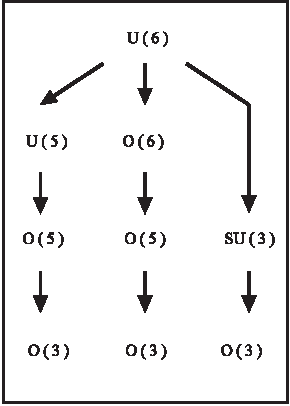
\includegraphics[scale=.65]{figure}
%
% If not, use
%\picplace{5cm}{2cm} % Give the correct figure height and width in cm
%
\caption{Please write your figure caption here}
\label{fig:A1}       % Give a unique label
\end{figure}

% For tables use
\begin{table}
\caption{Please write your table caption here}
\label{tab:A1}       % Give a unique label
%
% For LaTeX tables use
%
\begin{tabular}{p{2cm}p{2.4cm}p{2cm}p{4.9cm}}
\hline\noalign{\smallskip}
Classes & Subclass & Length & Action Mechanism  \\
\noalign{\smallskip}\hline\noalign{\smallskip}
Translation & mRNA$^a$  & 22 (19--25) & Translation repression, mRNA cleavage\\
Translation & mRNA cleavage & 21 & mRNA cleavage\\
Translation & mRNA  & 21--22 & mRNA cleavage\\
Translation & mRNA  & 24--26 & Histone and DNA Modification\\
\noalign{\smallskip}\hline\noalign{\smallskip}
\end{tabular}
$^a$ Table foot note (with superscript)
\end{table}
%


%%%%%%%%%%%%%%%%%%%%%%%%%%%%%%%%%%%%%%%%%%%%%%%%%%%%%%%%%%%%%%%%%%%%%%

\end{document}





